\chapter{Graphics}

\section{Sprite}
	Each Sprite consists of an image. The sprite have a display time (in seconds, double), and one collision box with scenary. If none collision box is provided, the entire sprite is a collision box as shows Figure \ref{spriteCollisionBox}.
	
	Each sprite may have a set of collision boxes where is vulnerable and a set of collision boxes where is attacking.
	
	\begin{figure}[H]
		\centering
		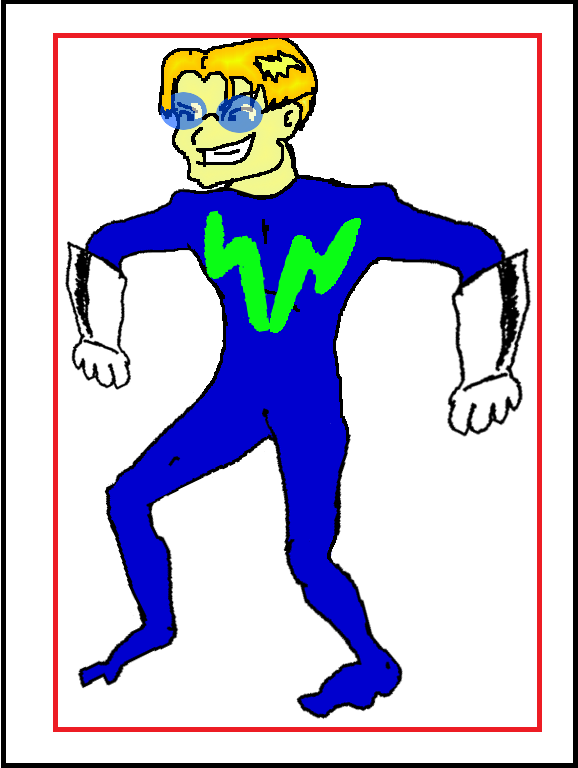
\includegraphics[width=0.45 \textwidth] {img/colisionbox.png}
		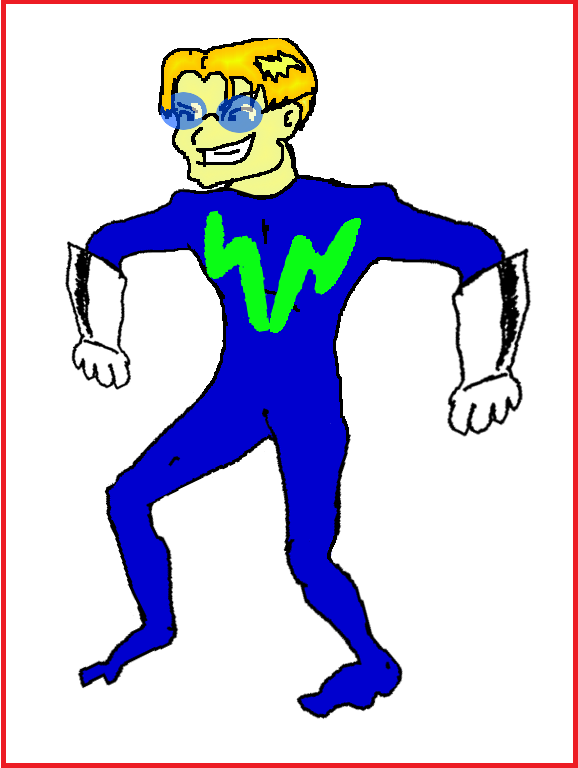
\includegraphics[width=0.45 \textwidth] {img/nocolisionbox.png}
		\caption {Sprite with an collision box (left, in red), and without defining an collision box (right, red).}
		\label{spriteCollisionBox}
	\end{figure}

	\subsection{Drawing the Sprite}
	All Sprite are drawin from the bottom of the point (MIDDLE, 0). The position of the character marks it position and the character is drawn based in this position as shows Figure \ref{fig:spriteDraw}.
	
	\begin{figure}[H]
		\centering
		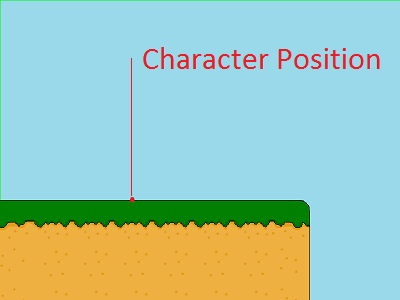
\includegraphics[width=0.32 \textwidth] {img/spritedraw0.png}
		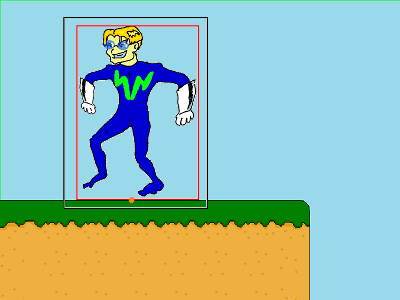
\includegraphics[width=0.32 \textwidth] {img/spritedraw1.png}
		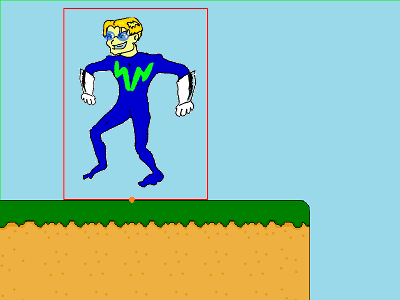
\includegraphics[width=0.32 \textwidth] {img/spritedraw2.png}
		\caption {Positioning the sprite in the character position.}
		\label{fig:spriteDraw}
	\end{figure}
	
	Thus, we can see that it is recommended to always make all sprite animation centering the sprites, and make all character and enemies sprites with the same size.
	
	\subsection{Sprite Coordinate System}
	The Sprite coordinate system is inverse to the bitmaps coordinate system. The (0,0) point is the lower left corner and the (W,H) point is the upper right point as shows Figure \ref{}.
	
	\section{Window \& Drawing}
	The game can support multiple resolutions. Before draw the game to the computer screen it is drawn to a buffer. 
	\textbf{ALL GRAPHIC DATA MUST BE CREATED USING THE INTERNAL RESOLUTION}. Table \ref{} shows the recommended size of graphics and the size of internal window. All data is drawn to the buffer and the buffer is resized in order to fill the screen as can be seen in Figure \ref{fig:display}.
	
	\section{Rendering}
	The Interface \emph{render.Renderable} is used in the \emph{render.Render} class. This Interface  has one method \emph{render(Graphics2D g)} wich takes one argument. This argument is the draw buffer in the size of the internal window. All objects that will be rendered must implement this method. In the GameManager these objects must be put in the render queue -- the Render access the \emph{render} method of all objects in depth order. The usuar order to draw is  Background, Scenary, character (playabe and enemies) and items, and, at last the Head Up Display (HUD).
	
	